 \documentclass[12pt]{article}
\usepackage{graphicx} % for inserting images
\usepackage[utf8]{inputenc} % for good practice
\usepackage{amsmath} % for equations
\usepackage{amsfonts}
\usepackage{hyperref}
\usepackage[ruled,linesnumbered]{algorithm2e}
\usepackage{setspace}
\usepackage{siunitx}
\sisetup{output-exponent-marker=\ensuremath{\mathrm{e}}}

\newcommand{\norm}[1]{\left\lVert#1\right\rVert}

\title{Support Vector Regression\\using\\Deflected Subgradient Methods}
\author{FearEP\\Lord Gugger}
\begin{document}
	\begin{titlepage}
		\maketitle
		\pagenumbering{gobble}
			%\pagenumbering{arabic} per rimettere i numeri
	   \begin{center}
		\vspace{0.5cm}
	        \textit{A project presented for the\\Computational Mathematics for Learning and Data Analysis\\course}
	       \vfill	     
	       
\includegraphics[width=0.2\textwidth]{unipi.png}\\
	       University of Pisa\\
	       Artificial Intelligence\\
			A.Y. 2020/2021\\
	            
	   \end{center}
	\end{titlepage}
	
	\newpage
	\begin{abstract}
		 Project aim is developing the implementation of a model which follows an SVR-type approach including various different kernels. The implementation uses as optimization algorithm a dual approach with appropriate choices of the constraints to be dualized, where the Lagrangian Dual is solved by an algorithm of the class of deflected subgradient methods.
	\end{abstract}
	
	\section{Introduction}
Per affrontare questo problema di regressione ci vogliamo affidare ad un modello di apprendimento supervisionato che è il Support Vector Regression. SVR ha come obiettivo trovare una funzione tale per cui ogni record assegnatoci per il training non devii da essa più di  $\varepsilon$  (per questo ogni valore all’interno del cosiddetto $\varepsilon$-tube non viene considerato come errore nella fase di ottimizzazione, rendendo la loss del modello $\varepsilon$-insensitive). Per fare ciò abbiamo bisogno di un certo parametro C (per capire il livello di regolarizzazione che desideriamo) ed un valore $\varepsilon$ (per esprimere l’errore che accettiamo), oltre ad eventuali parametri necessari ad attuare i kernel (e.g. gamma per quanto riguarda il kernel RBF). Parte fondante del modello, oltre a ciò sopra descritto riguardo l’ $\varepsilon$-tube, è dare allo stesso tempo importanza al mantenere la funzione \textit{as flat as possible}, per evitare overfitting ed avere dunque un modello che sia un corretto tradeoff tra accuratezza e generalità.
	\begin{figure}[h]
		\centering
		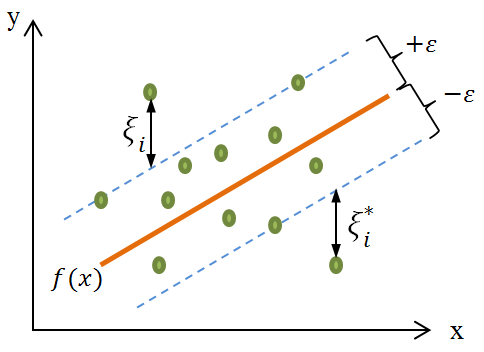
\includegraphics[width=0.5\textwidth]{svrIntro}
		\caption{a generic svr}
		\label{fig:svr_intro}
	\end{figure}

La funzione risultante dall’ottimizzazione del modello è descritta genericamente come:

	\begin{equation}\label{eq:0}
		f(x) = w  x + b
	\end{equation}

Obiettivo dell’ottimizzazione è dunque fare in modo che la curva sia, di nuovo, \textit{as flat as possible}, ma questo è equivalente ad un problema di ottimizzazione dove vogliamo avere $\norm{w}$ minima. 
Per comodità di formulazione del problema possiamo minimizzare $\norm{w}^2$ senza cambiare il significato. Questo ci permette di portarci in un problema di ottimizzazione quadratico, grazie al quale potremo approfittare del concetto di \textbf{strong duality} più tardi. 
Introduciamo a questo punto delle variabili dette \textit{slack} per formulare la \textit{dual objective function}, la quale rappresenta il nostro \textit{primal problem}:
	\begin{equation}\label{eq:1}
		\min_{w,b,\xi_i,\xi_i^*} \frac{1}{2}\norm{w}^2+C\sum_{i}(\xi_{i} + \xi_{i}^*)
	\end{equation}
	Ciò che viene sommato a $\norm{w}$ è un elemento che ci permette di regolare l’errore, e di conseguenza la penalità, dovuti alla possibile presenza di elementi che non rimangono all’interno dell’ $\varepsilon$-tube. Vediamo dunque come C funga da regolarizzatore in una metodica simile a L1. I vari $\xi$ vengono detti \textit{slack variables} e ci permettono di definire i vincoli del problema per qualsiasi i-esimo dato:

	\begin{equation}\label{eq:2}
	\begin{aligned}
		&y_i - w^T\phi(x_i) - b \leq \epsilon + \xi_i,  \\ 
		&b + w^T\phi(x_i) - y_i \leq \epsilon + \xi_i, \\
		&\xi_i,\xi_i^*  \geq 0
	\end{aligned}
	\end{equation}

	\begin{center}
		\footnotesize{x i-esimo input, y i-esimo output}
	\end{center}
	
	Essendo in un problema di ottimizzazione quadratico, la soluzione al \textit{dual problem} risulta equivalente a quella del \textit{primal problem}. In particolare in questa casistica risulta più facile la risoluzione del \textit{dual problem} vista la possibile applicazione del concetto di kernel. Costruiamo dunque il \textit{dual problem} definendo la relativa Lagrangiana (equivalente del \textit{primal problem} al quale aggiungiamo i vincoli sommandoli o sottraendoli):
	

	\begin{equation}\label{eq:3}
	\begin{aligned}
		L(\alpha,\alpha^*,\mu,\mu^*) =  \ &\frac{1}{2}\norm{w}^2\\
		&+C\sum_{i=1}^{m}(\xi_{i} + \xi_{i}^*) \\
		&+ \sum_{i=1}^{m}(\alpha_i(y_i - w^T\phi(x_i) - b - \epsilon - \xi_i))\\
		&+ \sum_{i=1}^{m}(\alpha_i^*(w^T\phi(x_i) + b - y_i - \epsilon - \xi_i^*)) \\
		\sum_{i=1}^{m}(\mu_i\xi_i + \mu_i^*\xi_i^*)
	\end{aligned}
	\end{equation}

	A causa del concetto di \textbf{\textit{weak duality}} qualsiasi valore del \textit{primal problem} risulta maggiore (o uguale) del \textit{dual problem}. Da questa considerazione deriviamo il fatto che il punto di massima vicinanza tra i 2 problemi è dove il \textit{primal problem} ha minimo e il \textit{dual problem} ha massimo. Nella casistica di \textit{strong duality} questa vicinanza si tramuta uguaglianza.
Cerchiamo dunque di rielaborare il \textit{dual problem} per lavorare con meno variabili possibili, in particolare eliminiamo dai calcoli la variabile w, b e le 2 \textit{slack} $\xi$ e $\xi^*$. In che modo? Stiamo cercando un valore ottimo che tra l’altro sarà unico data la casistica quadratica, dunque la derivata parziale relativa ad ognuna di queste variabili va posta a 0. Questo ci porta a poter ridefinire w:

	\begin{equation}\label{eq:4}
		w = \sum_{i=1}^{m}(\alpha_i - \alpha_i^*)\phi(x_i)
	\end{equation}

	Infine tramite sostituzione nella Lagrangiana definita precedentemente arriviamo ad una funzione dipendente solamente da $\alpha$ e $\alpha^*$:

	\begin{equation}\label{eq:5}
	\begin{aligned}
		\max_{\alpha_i,\alpha_i^*} &- \frac{1}{2}\sum_i\sum_j(\alpha_i - \alpha_i^*)(\alpha_j - \alpha_j^*)K(x_i,x_j) \\
		&- \epsilon\sum_i(\alpha_i + \alpha_i^*)\\
		&+ \sum_i y_i(\alpha_i - \alpha_i^*)
	\end{aligned}
	\end{equation}

	Notiamo che le uniche variabili rimaste sono i moltiplicatori lagrangiani $\alpha$ e $\alpha^*$, i quali sono sottoposti ai seguenti vincoli:
	
	\begin{equation}\label{eq:6}
		\begin{aligned}
		&\forall i \: \alpha_i,\alpha_i^* \geq 0 \qquad\qquad &&(KKT condition) \\
		&\forall i \: \alpha_i,\alpha_i^* \in [0,C]  \qquad\qquad &&(from \: deriving \: \eqref{eq:5})\\
		&\forall i \: \sum (\alpha_i - \alpha_i^*) = 0 \qquad\qquad &&(from \: deriving \: \eqref{eq:5})\\
		&\forall i \: \alpha_i \alpha_i^* = 0 \qquad\qquad &&(from \: model \: construction)
		\end{aligned}
	\end{equation}
			
%discorsi vari sui kernel

	Restando ancora su \eqref{eq:5}, approfondiamo l'elemento $K(x_i,x_j)$, ovvero ciò rappresenta il concetto di \textbf{kernel}, sostituendo ciò che sarebbe un prodotto scalare nello spazio necessitato. Rielaboriamo dunque la precedente frase: certi problemi di regressione non possono essere adeguatamente descritti da modelli lineari. Risulta dunque comodo cambiare spazio di visualizzazione, per portarci in un nuovo spazio (con ogni probabilità con più dimensioni rispetto allo spazio originale) dove il problema diventa linearmente affrontabile. Il cambio di base risulta essere incredibilmente dispendioso per il training del modello ed è proprio in questo caso che il kernel diventa il fulcro dell’efficienza di SVC/SVR. Ci permette infatti di eseguire il \textit{dot-product} nello spazio attuale ma avere come risultato il \textit{dot-product} nello spazio richiesto. Ci permette di risparmiare molte computazioni e di poterle riutilizzare salvandoci i valori risultanti in una \textit{kernel matrix} (riutilizzabile ad ogni ciclo di ottimizzazione). Ovviamente non c’è la certezza di aver preso in considerazione il kernel corretto per la casistica, bisognerà dunque svilupparne vari, magari certi funzioneranno meglio di altri (\textit{rbf, sigmoid, etc}).\\
In particolare questa implementazione prevede il possibile utilizzo di diversi kernel:\\
	\begin{itemize}
		\item linear: $\langle x,x' \rangle$
		\item polynomial: $(\gamma\langle x,x' \rangle + r)^d$
		\item rbf: $\exp(-\frac{\norm{x \  x'}^2}{2\sigma^2})$
		\item sigmoid: $\tanh(\gamma\langle x,x' \rangle + r)$
	\end{itemize}

%discorsi parte finale post definizione problema
	Definito il problema possiamo a questo punto cercare il massimo del \textit{dual problem}. La task da noi scelta utilizzerà \textbf{deflected subgradient methods} per raggiungere l’obiettivo. Una volta raggiunto il massimo avremo a nostra disposizione i corretti $\alpha$ e $\alpha^*$ necessari per il calcolo di w. 

	Per completare la funzione risolutrice del problema ci basta trovare il parametro b. Ricavarlo risulta semplice una volta preso in considerazione un qualsiasi elemento del nostro insieme di input tale per cui la relativa predizione (y i-esimo) sia al limite dell’ $\varepsilon$-tube o al di fuori di esso. Proprio quell’insieme di valori sarà infatti l’unico ad avere come vincoli attivi almeno uno tra i vari $\alpha$ e $\alpha^*$, ovvero un $\alpha$ o $\alpha^*$ diversi da 0. Essendo dunque al margine di un vincolo potremo, derivando da \eqref{eq:0} e \eqref{eq:4}:

	\begin{equation*}
		x_j \  with\  \alpha_j \in(0,C): b = y_j - \sum_i(\alpha_i - \alpha_i^*)K(x_i,x_j)
	\end{equation*}

	Una volta trovata la funzione risultante possiamo testare la bontà del modello effettuando \textit{prediction} su un set di test input per poi calcolare la metrica MSE tra output previsto dal modello e output effettivo del set di test input.\\
Questo fatto è particolarmente importante per il confronto tra modelli e dunque per la ricerca dei parametri migliori possibili (\textit{grid search}).


	\section{Structures for implementation}
	\begin{itemize}
		\item kernel matrix: presi $m$ record di input sarà una matrice simmetrica $ K(x,x') \in \mathbb{R}^{m,m}$
		\item alpha matrix: presi $m$ record di input sarà un vettore $ A \in \mathbb{R}^{2m} $ tale per cui $A_i \neq 0$ solo se il relativo input genera un output che contribuisce alla $loss$ . Prima metà di $A$ rappresenterà l'insieme di $\alpha$ mentre la seconda metà rappresenterà l'insieme di $\alpha*$ .
	\end{itemize}

	\section{Algorithm introduction}
	Qui parleremo del Deflected, magari spiegando un attimo il Target Level, Polyak e constraint vari tra $\beta$ e $\gamma$.

	\section{Pseudo Code}
	\begin{algorithm}[H]
		\DontPrintSemicolon
		\KwIn{$X$ input matrix of size $m \times d$ \newline
			$y$  output vector of size $m$\newline
			$C$ regularization parameter\newline
			$\varepsilon$  parameter defining sensitiveness of model\newline
			$kernel\_type$ defining which kernel to use\newline
			$args$ necessary and different for each kernel}
		\KwOut{Parameters $w$ e $b$ for resulting function ( $ f(x) = wx + b $ )}
		\setstretch{1.35}
		
		\Begin{
			$K \longleftarrow kernel(X, kernel\_type, args)$\\
			\tcp{to assure $Q$ to be Positive Semidefinite}
			$Q \longleftarrow [K\qquad -K ;\qquad -K \qquad\;  K]$\\
			$q \longleftarrow [-y\qquad y]$\\
			$q \longleftarrow q + \varepsilon$\\
			$upper\_bound \longleftarrow C$\\
			$alphas \longleftarrow Fit\_SVR(Q,q,upper\_bound)$\\
			$alpha^+ \longleftarrow alphas_{0:(size(alphas)/2)}$\\
			$alpha^- \longleftarrow alphas_{(size(alphas)/2):size(alphas)}$\\
			$w \longleftarrow (alpha^+ - alpha^-)K$\\
			\tcp{find first $alpha^+$ or $alpha^- \ne 0$ and save index in $alpha\_not\_zero$}
			$b = y_{alpha\_not\_zero} - \sum_i (alpha^+_i - alpha^-_i)K_{i,alpha\_not\_zero}$\\
		}
		 \caption{Get\_SVR}
	\end{algorithm}
	

	
	Discussione su algoritmo, discorso su Q e su b.\\



	\begin{algorithm}[H]
		\DontPrintSemicolon
		\KwIn{$Q$ input matrix of size $2m \times 2m$ \newline
		$q$  output vector of size $2m$\newline
		$ub$ upper bound for constrained variables\newline
		$stopping\_criterion$ $(default = \num{1e-12})$\newline
		$\gamma$ for Target Level $(default = 0.5)$\newline
		$\beta$ for Target Level $(default = 0.5)$\newline
		$eps$ for Target Level $(default = \num{1e-6})$\newline
		$\delta\_reset$ for Target Level $(default = \num{1e-4})$\newline
		$\rho$ for Target Level $(default = 0.95)$
		}
			
		\KwOut{Optimal $x$ to minimize constrained $\frac{1}{2}x'Qx + qx$}
		\setstretch{1.35}
		
		\Begin{
		$x \longleftarrow ([0] \times size(q))'$\\
		$xref \longleftarrow x$\\
		$fref \longleftarrow inf$\\
		$\delta\_prev \longleftarrow 0$\\
		$iter \longleftarrow 1$\\
		$\delta \longleftarrow 0$\\
		}
		 \caption{Fit\_SVR}
	\end{algorithm}

\end{document}